\documentclass[a4paper,9pt]{scrartcl}
\usepackage[utf8]{inputenc}
\usepackage[T1]{fontenc}
\usepackage{graphicx}
\usepackage{xcolor}
\usepackage[yyyymmdd,hhmmss]{datetime}
\usepackage{subfigure}
\usepackage[top=0.5in, bottom=1in, left=0.4in, right=0.4in]{geometry}
\usepackage{multicol}
\newenvironment{Figure}
  {\par\medskip\noindent\minipage{\linewidth}}
  {\endminipage\par\medskip}

\title{\vspace{-7ex}Analysis of FlexCast Reconfiguration}
\date{\vspace{-10ex}}
\begin{document}
\maketitle


%%%%%%%%%%%%%%%%%%%%%%%%%%%%%%%%%%%%%%%%%%%%%%%%%%%%

\section{Experiment Config.}
\begin{multicols}{3}
    \small
    \begin{itemize}
        \item \textbf{TPCC/AWS Latencies}
        \item \textbf{Exp. Duration:} 2 min
        \item \textbf{Reconfig interval:} 30sec
    \end{itemize}
    \columnbreak
    \begin{itemize}
    	\small
        \item \textbf{Regions/Nodes: 3}  \\(Calif., Virg., Sao Paulo)
        \item \textbf{Clients: 150} (50 per region)
        \item \textbf{Locality: 95\%}
    \end{itemize}
    \columnbreak
    \begin{Figure}
        \centering
        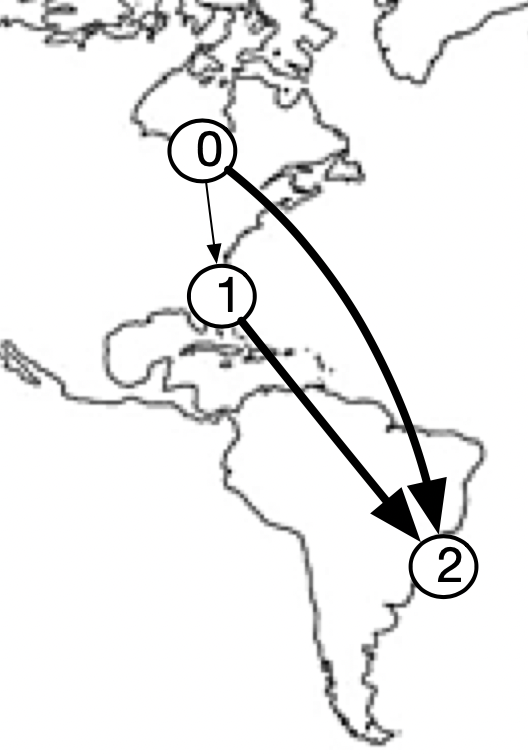
\includegraphics[scale=.29]{figs/CVS.png}
    \end{Figure}
\end{multicols}

\section{Results}
\small
\begin{multicols}{2}
    \subsection{Throughput}
    \begin{Figure}
        \centering
        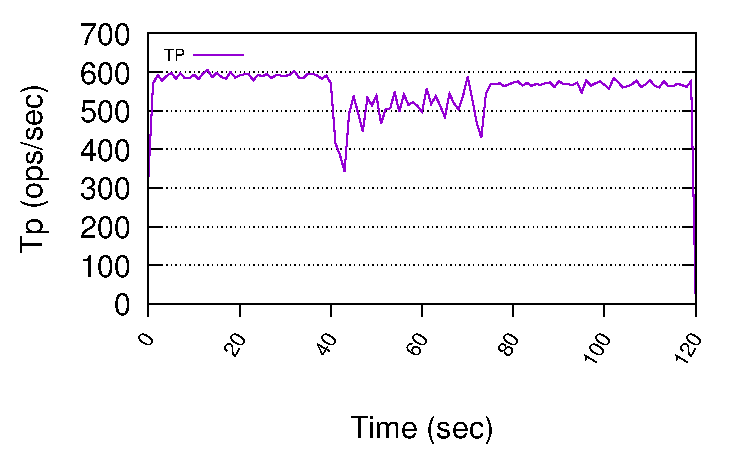
\includegraphics[scale=.5]{figs/3nodesCVS/tp95.pdf}
    \end{Figure}
    \columnbreak
    \subsection{Latency}
    \begin{Figure}
        \centering
        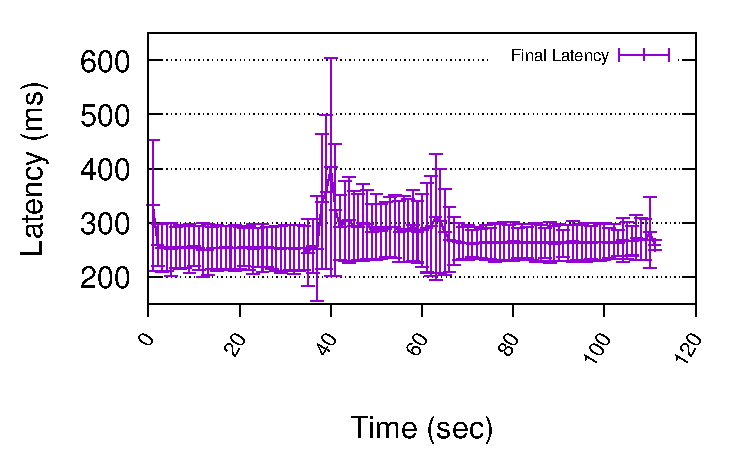
\includegraphics[scale=.5]{figs/3nodesCVS/lat95.pdf}
    \end{Figure}
\end{multicols}

\subsection{Reconfiguration details}

\begin{multicols}{4}
\footnotesize

\begin{verbatim}
workload 1 : [
    {
        "destination": [0, 1],
        "percentage": 0.032794576
    },
    {
        "destination": [0, 2],
        "percentage": 0.57712483
    },
    {
        "destination": [0, 1, 2],
        "percentage": 0.050535202
    },
    {
        "destination": [1, 2],
        "percentage": 0.3395454
    },
]
Took 55 ms 
\end{verbatim}
\columnbreak
\begin{Figure}
    \centering
    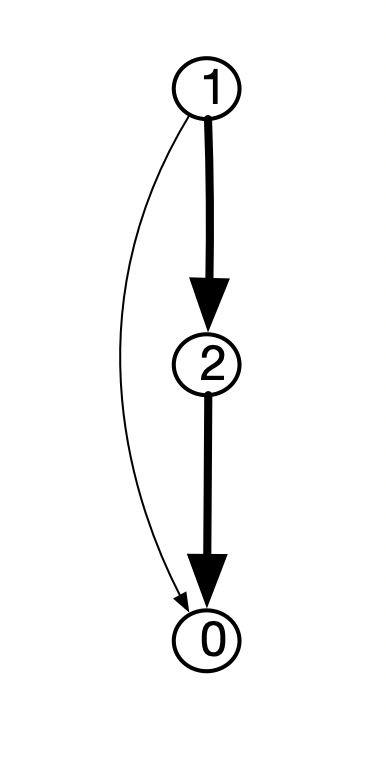
\includegraphics[scale=.3]{figs/3nodesCVS/reconfig1.png}
\end{Figure}

\columnbreak

\begin{verbatim}
workload 2 : [
    {
        "destination": [1, 2, 0],
        "percentage": 0.05174473
    },
    {
        "destination": [2, 0],
        "percentage": 0.5442484
    },
    {
        "destination": [1, 0],
        "percentage": 0.034562822
    },
    {
        "destination": [1, 2],
        "percentage": 0.36944407
    },
]
Took 5 ms 
\end{verbatim}
\begin{Figure}
    \centering
    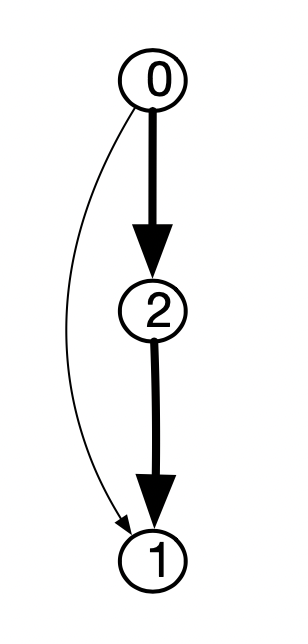
\includegraphics[scale=.3]{figs/3nodesCVS/reconfig2.png}
\end{Figure}

\columnbreak

\end{multicols}

\subsection{Latencies per dests}

\begin{Figure}
    \centering
    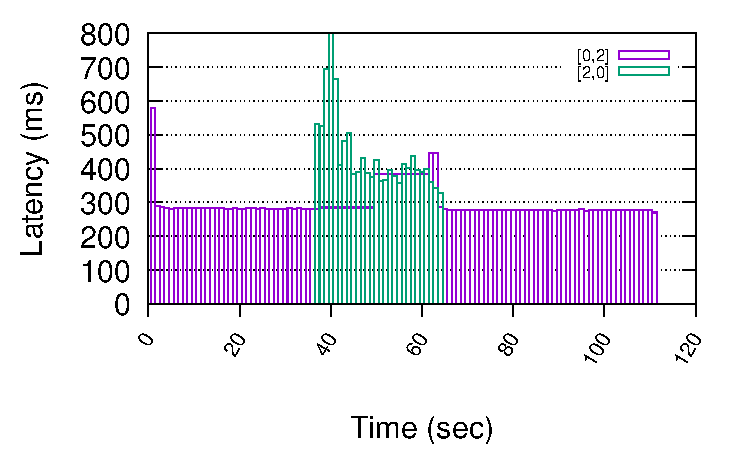
\includegraphics[page=1, scale=.5]{figs/3nodesCVS/latperdest95p.pdf}
    \includegraphics[page=2, scale=.5]{figs/3nodesCVS/latperdest95p.pdf}
    \includegraphics[page=3, scale=.5]{figs/3nodesCVS/latperdest95p.pdf}
    \includegraphics[page=4, scale=.5]{figs/3nodesCVS/latperdest95p.pdf}
\end{Figure}

\newpage

%%%%%%%%%%%%%%%%%%%%%%%%%%%%%%%%%%%%%%%%%%%%%%%%%%%%



\section{Experiment Config.}
\begin{multicols}{3}
    \small
    \begin{itemize}
        \item \large \textbf{\color{red} NO CLIENT LATENCIES}
        \item \textbf{TPCC/AWS Latencies}
        \item \textbf{Exp. Duration:} 2 min
        \item \textbf{Reconfig interval:} 30sec
    \end{itemize}
    \columnbreak
    \begin{itemize}
    	\small
        \item \textbf{Regions/Nodes: 3}  \\(Calif., Virg., Sao Paulo)
        \item \textbf{Clients: 150} (50 per region)
        \item \textbf{Locality: 95\%}
    \end{itemize}
    \columnbreak
    \begin{Figure}
        \centering
        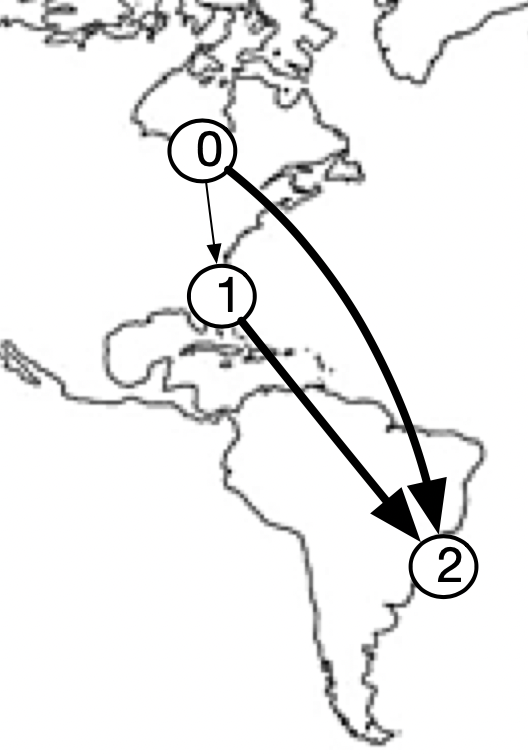
\includegraphics[scale=.33]{figs/CVS.png}
    \end{Figure}
\end{multicols}

\section{Results}
\small
\begin{multicols}{2}
    \subsection{Throughput}
    \begin{Figure}
        \centering
        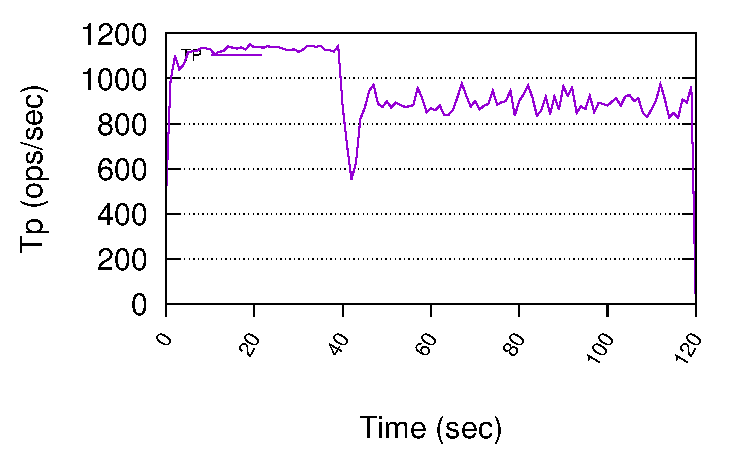
\includegraphics[scale=.5]{figs/3nodesCVS/noclilat-tp95.pdf}
    \end{Figure}
    \columnbreak
    \subsection{Latency}
    \begin{Figure}
        \centering
        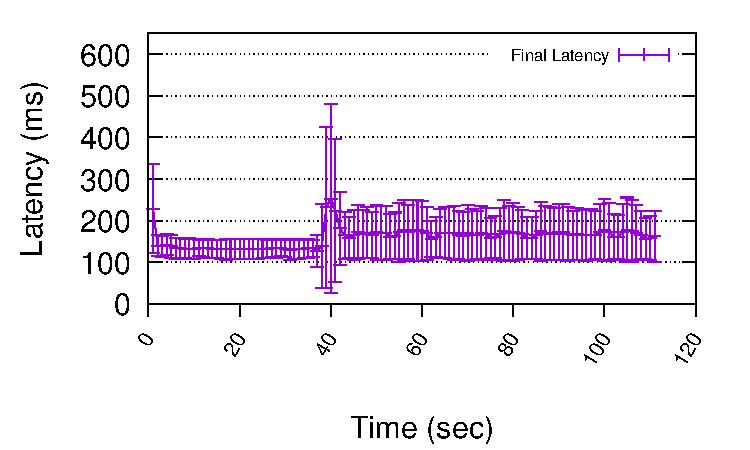
\includegraphics[scale=.5]{figs/3nodesCVS/noclilat-lat95.pdf}
    \end{Figure}
\end{multicols}

\subsection{Reconfiguration details}

\begin{multicols}{2}
\footnotesize

\begin{verbatim}
workload 1 : [
    {
        "destination": [0, 1],
        "percentage": 0.03268678
    },
    {
        "destination": [0, 2],
        "percentage": 0.5705819
    },
    {
        "destination": [0, 1, 2],
        "percentage": 0.052015986
    },
    {
        "destination": [1, 2],
        "percentage": 0.34471536
    },
]
Took 55 ms 
\end{verbatim}
\columnbreak
\begin{Figure}
    \centering
    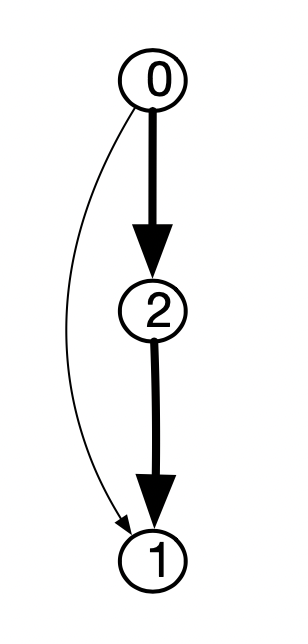
\includegraphics[scale=.5]{figs/3nodesCVS/reconfig2.png}
\end{Figure}

\end{multicols}

\subsection{Latencies per dests}

\begin{Figure}
    \centering
    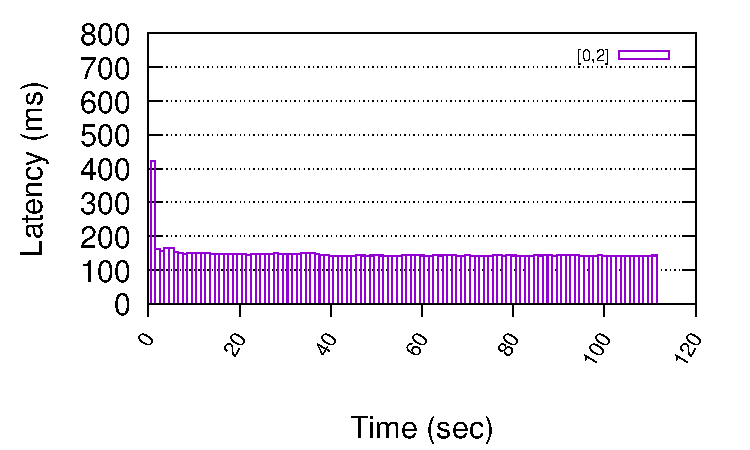
\includegraphics[page=1, scale=.5]{figs/3nodesCVS/noclilat-lat95-perdest90p.pdf}
    \includegraphics[page=2, scale=.5]{figs/3nodesCVS/noclilat-lat95-perdest90p.pdf}
    \includegraphics[page=3, scale=.5]{figs/3nodesCVS/noclilat-lat95-perdest90p.pdf}
    \includegraphics[page=4, scale=.5]{figs/3nodesCVS/noclilat-lat95-perdest90p.pdf}
\end{Figure}

\newpage
%%%%%%%%%%%%%%%%%%%%%%%%%%



% \section{Experiment Config.}
% \begin{multicols}{3}
%     \begin{itemize}
%         \item \textbf{TPCC/AWS Latencies}
%         \item \textbf{Exp. Duration:} 2 min
%         \item \textbf{Reconfig interval:} 40sec
%     \end{itemize}
%     \columnbreak
%     \begin{itemize}
%     	\small
%         \item \textbf{Regions/Nodes: 3}  \\(Virg., Frank., Mumbai)
%         \item \textbf{Clients: 150} (50 per region)
%         \item \textbf{Locality: 95\%}
%     \end{itemize}
%     \columnbreak
%     \begin{Figure}
%         \centering
%         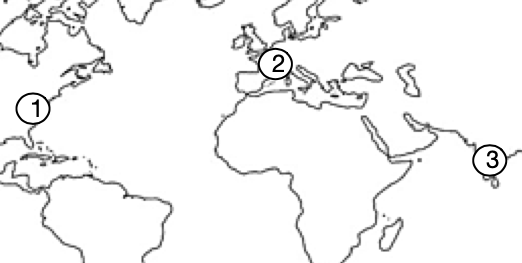
\includegraphics[scale=.3]{figs/VFM.png}
%     \end{Figure}
% \end{multicols}

% \section{Results}

% \begin{multicols}{2}
%     \subsection{Throughput}
%     \columnbreak
%     \subsection{Latency}
% \end{multicols}

% \subsection{Reconfiguration}

% %%%%%%%%%%%%%%%%%%%%%%%%%%%%%%%%%%%%%%%%%%%%%%%%%%%%

% \newpage
% \section{Experiment Config.}
% \begin{multicols}{3}
%     \begin{itemize}
%         \item \textbf{TPCC/AWS Latencies}
%         \item \textbf{Exp. Duration:} 2 min
%         \item \textbf{Reconfig interval:} 40sec
%     \end{itemize}
%     \columnbreak
%     \begin{itemize}
%     	\small
%         \item \textbf{Regions/Nodes: 6}
%         \item \textbf{Clients: 150} (50 per region)
%         \item \textbf{Locality: 95\%}
%     \end{itemize}
%     \columnbreak
%     \begin{Figure}
%         \centering
%         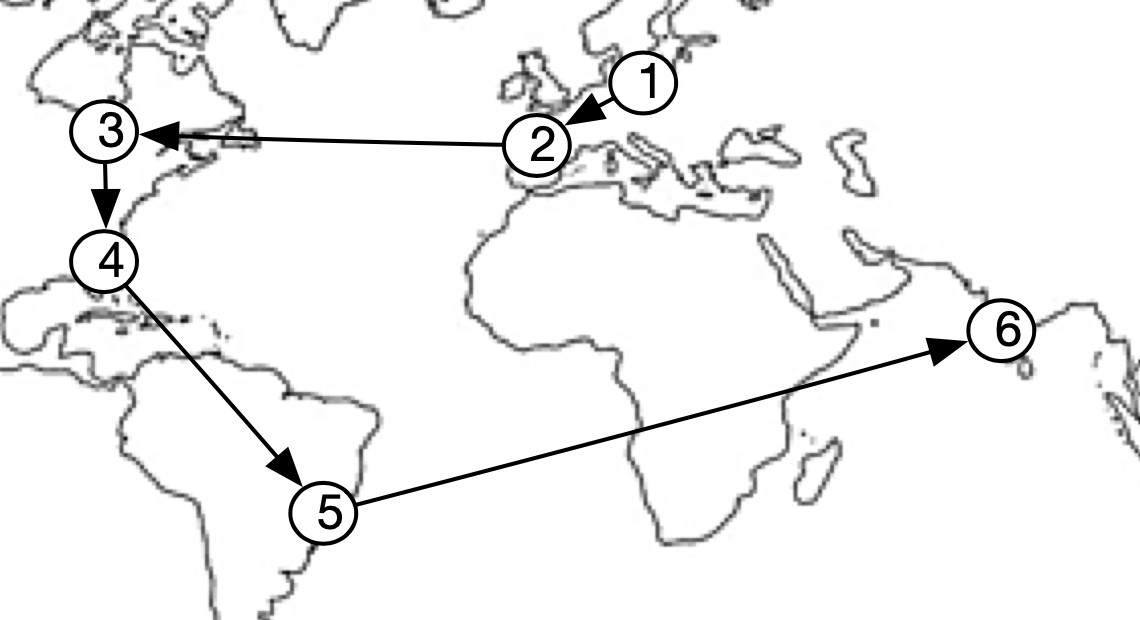
\includegraphics[scale=.3]{figs/6nodes.png}
%     \end{Figure}
% \end{multicols}

% \section{Results}

% \begin{multicols}{2}
%     \subsection{Throughput}
%     \columnbreak
%     \subsection{Latency}
% \end{multicols}

% \subsection{Reconfiguration}

\end{document}
